\section{\acs{led} osvětlení}
\label{sec:perif-led-osvetleni}

    Úkolem této periferie je zajistit osvětlení akvária a umožnit jeho ovládání. V porovnání s ostatními moduly je zapojení relativně komplexní a proto byla pro tuto periferii navržena a zhotovena vlastní \acs{dps} (fungující jako dceřinná deska, viz.~\ref{sec:modul-periferie}). Jako typ svítidla byly zvoleny \acs{led} pásky pracující s napětím \qty{12}{V}. Modul musí být schopen samostatně ovládat 2 \acs{led} pásky, kdy za pomocí regulace proudu do \acs{led} pásku nastaví intenzitu osvětlení. 

\subsection{Návrh zapojení}
    Na začátku návrhu je potřeba specifikovat si požadavky na elektrické parametry zapojení. Uvažujme délku každého pásku \(l=\qty{1}{m}\), vstupní napětí získané z konektoru D-sub \(U_{in} =\qty{24}{V}\) a výstupní napětí pro které je pásek určen \(U_{out} =\qty{12}{V}\). Pro stanovení maximálního proudu bylo vycházeno z údajů na e-shopu \acs{led} Solution~\cite{eshop-ledsolution-svetlo}, kdy nejvýkonější nabízený \acs{led} pásek pro dané napětí má příkon \(P_{i}= \qty{20}{W/m}\). Pak každý kanál musí být schopen dodat proud odpovídající nejnáročnějšímu scéáři:
    \begin{equation}  
        I_{max} = \frac{P_{i}\cdot l }{U_{out}} = \frac{20\cdot 1 }{12} = \qty{1.66}{A}
    \end{equation}

    Jelikož se jedná o dceřinnou desku pro obecný modul, rozměr výsledné \acs{dps} je omezen a část plochy je navíc využita konektory pro vsazení do obecného modulu. Je tedy potřeba zvolit co nejvíce integrované řešení, které současně slibuje dobrou účinnost a tedy co nejnižší ohřev zařízení během provozu.

    Pro řízení \acs{led} osvětlení je často používán proudový zdroj, který umožňuje lineárně regulovat výstupní proud a tím i intenzitu osvětlení. Na trhu existuje opět celá řada čipů určena přímo k ovládání \acs{led} pásků~\cite{TI_\acs{led}_Drivers}, problém je zde ale v tom, že uživatel velmi pravděpodobně připojí pásek s nižším, předem neznámým příkonem. Maximální proud je tedy specifický danému \acs{led} pásku a proudový zdroj by musel zároveň spolehlivě zaručit, že nebude překročeno napětí \(U_{out} =\qty{12}{V} \).

    Touto funkcí většina čipů nedisponuje a pokud ano, nejsou dostatečně integrované pro použití v této aplikaci. Po důkladné rešerši a několika iteracích návrhu se nakonec jeví jako nejlepší použití napěťového měniče typu buck spolu se zesilovačem pro snímání proudu. Snímaný proud je následně zpracován mikrokontrolérem a jsou upraveny poměry ve zpětné vazbě měniče, aby napětí odpovídalo požadovanému proudu.

    \begin{figure}[h!]
        \centering
        % trim=left bottom right top
        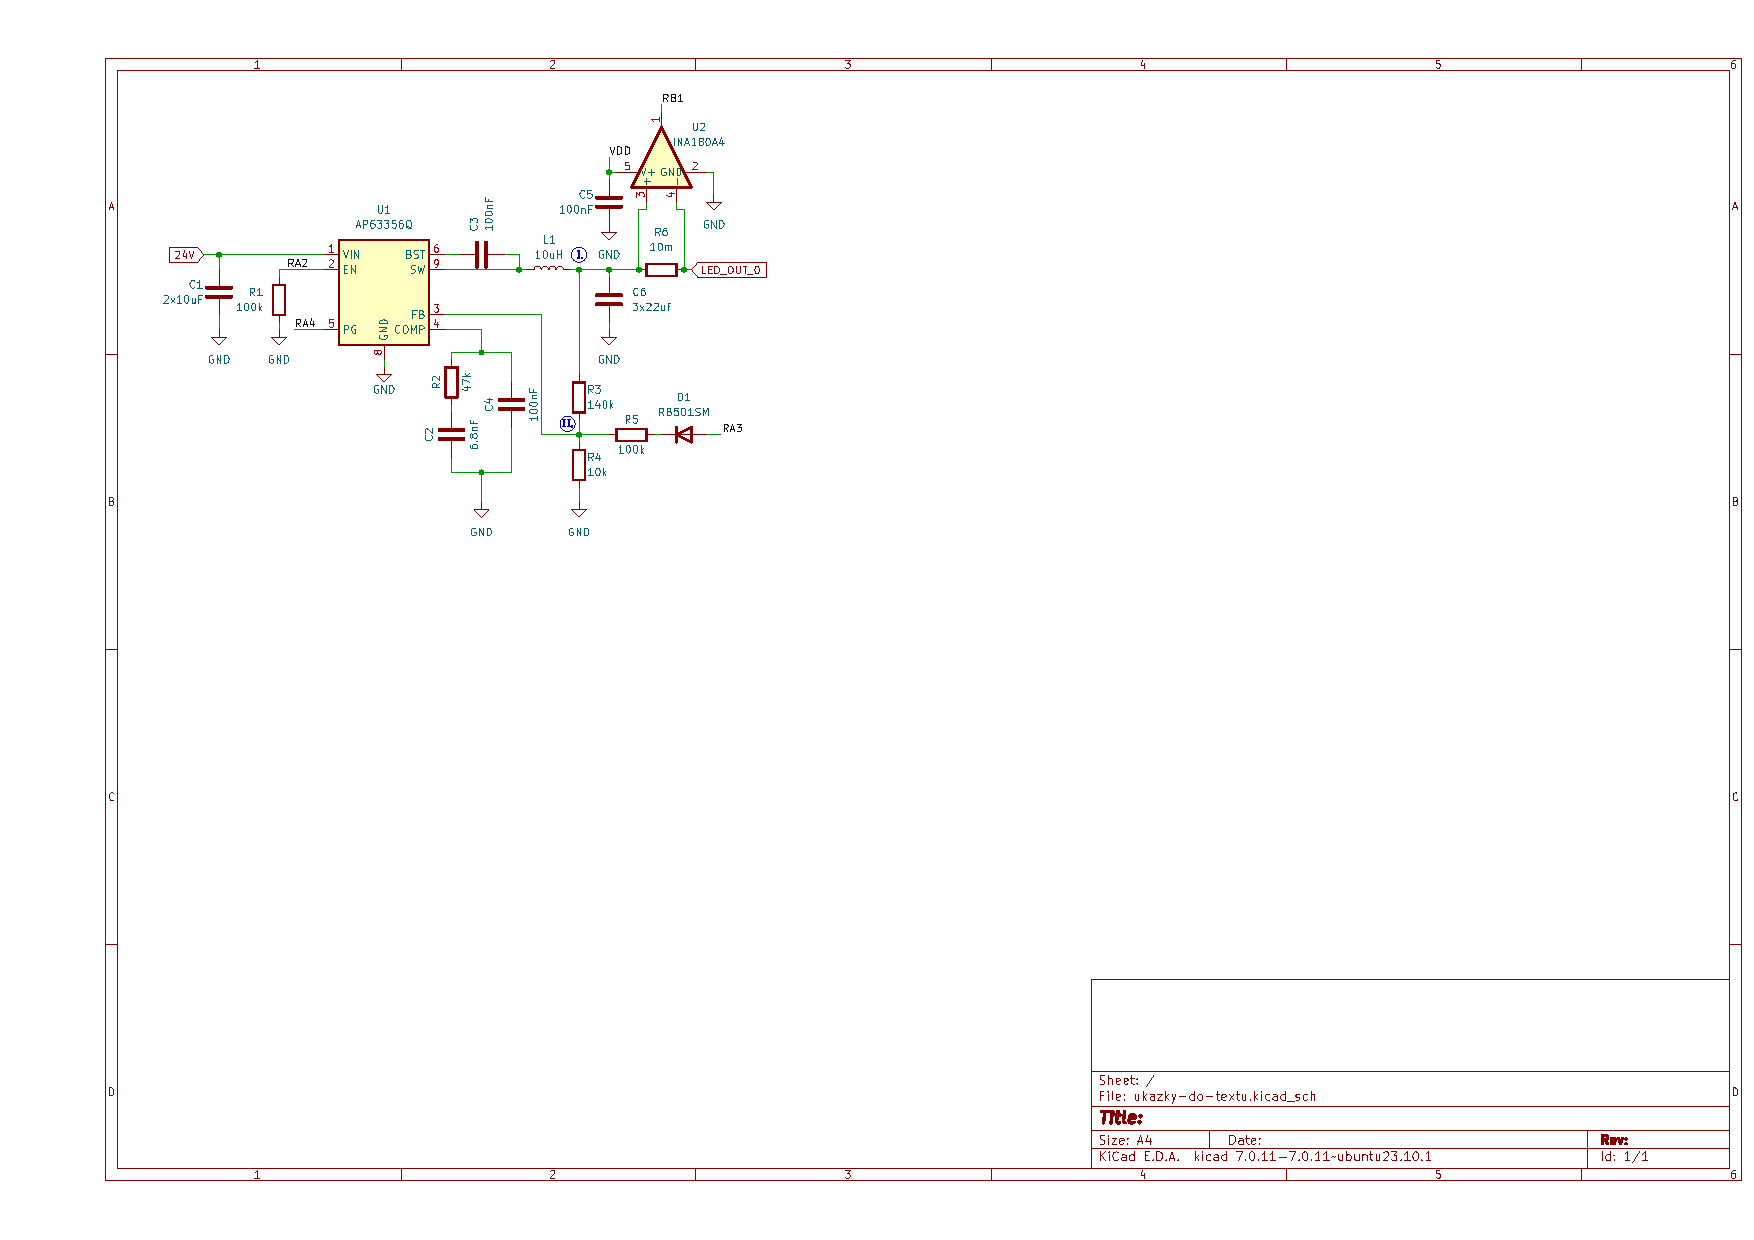
\includegraphics
        [
            width=\textwidth, 
            page=1, 
            trim=2.5cm 11.5cm 16cm 1.5cm, 
            clip
        ]{obrazky/exportovane/ukazky-do-textu.pdf}
        \caption{Zjednodušené schéma ovladače \acs{led}. Vytvořeno v~KiCad 7.0.}
        \label{fig:led-board-simp-schema}
    \end{figure}

    
\subsubsection{Popis schématu a výpočty hodnot součástek}
% TODO: projet ještě jednou poznámky od Pavla
    Zjednodušené schéma pro jeden ovládaný kanál se nachází na obr.~\ref{fig:led-board-simp-schema}, při výpočtech bude použito označení součástek z tohoto schématu. Úplné schéma modulu pak lze nalézt v příloze~\ref{priloha:schema-led-board}.

    Jako buck kontrolér je zvolen čip AP63356Q vyvinutý společností Diodes incorporated, jedná se o úspornou a velmi malou součástku, která v sobě integruje oba potřebné MOSFET tranzistory a spíná s pevně danou frekvencí \(f_{SW}=\qty{450}{kHz} \) ~\cite{Diodes_AP63356Q}. Pro snímání proudu poslouží čip INA180A4 firmy Texas Instruments~\cite{TI_INA180A4}.

    Z obrázku je vidět, že pro ovládání jednoho kanálu \acs{led} pásků jsou využity 4 piny \acs{mcu}, RA4 a RB1 fungují jako vstupy, RA2 a RA3 pak jako výstupy. Rezistor \(R_{1}\) drží buck měnič ve vypnutém stavu dokud mikrokontrolér nenastaví hodnotu pinu RA2 na logickou 1. Pin RA4 je pak čipem (\(U_{1} \)) stažen k zemi vždy, když na výstupu není odpovídající nastavené napětí.  
    
    Nastavení výstupního napětí měniče je dosaženo za pomoci zpětnovazební smyčky mezi výstupním uzlem (I.) a zpětnovazebním pinem FB (uzel II.). V uzlu II. je drženo konstantní napětí \qty{0.8}{V}~\cite{Diodes_AP63356Q}, poměrem rezistorů \(R_{3} \) a \(R_{4} \) je pak definováno výstupní napětí. Zvolíme hodnotu odporu \(R_{4} = \qty{10}{k\ohm}\), pro maximální požadované napětí \(U_{outMAX} = \qty{12}{V}\) platí:
    \begin{equation}
        R_{3} = R_{4}\cdot \left(\frac{U_{outMAX} }{\num{0.8}}-1\right) = \qty{10}{k}\cdot \left(\frac{12}{\num{0.8}}-1\right) = \qty{140}{k\ohm}
    \end{equation} 
    Na pin RA3 mikrokontroléru je přivedeno analogové napětí z periferie DAC popř. \acs{pwm} signál a skrze rezistor \(R_{5} \) (a ochrannou diodu) pak teče proud do rezistoru \(R_{4} \), úbytek napětí na tomto rezistoru je ale konstantní (\qty{0.8}{V}) a tedy je konstantní i proud rezistorem. Z prvního Kirchhoffova zákona pak víme, že proud rezistorem \(R_{3} \) klesne o hodnotu proudu dodanou z pinu RA3, tím klesne také napětí na výstupu měniče a dojde ke ztlumení jasu \acs{led} pásku. Citlivost (nebo také rozsah) změny je definován hodnotou \(R_{5} \), snížením jeho hodnoty lze dosáhnout na výstupu ještě nižšího napětí. Pro hodnotu \(R_{5} = \qty{100}{k\ohm}\) zobrazenou ve schématu lze nejnižší možné napětí vypočítat následovně:
    \begin{equation}
        U_{outMIN} = \num{0.8}+R_{3} \cdot I_{3} = \num{0.8}+R_{3} \cdot \left(\frac{\num{0.8}}{R_{4}} - \frac{U_{VDD} - U_{D1}}{R_{4}+R_{5}} \right) 
    \end{equation}  
    Kdy \(U_{VDD} = \qty{3.3}{V}\) je maximální napetí pinu RA3 a \(U_{D1}=\qty{0.35}{V} \) je prahové napětí zvolené diody. Po dosazení získáme:
    \begin{equation}
        U_{outMIN} = \num{0.8}+\qty{140}{k} \cdot \left(\frac{\num{0.8}}{\qty{10}{k}} - \frac{\num{3.3} - \num{0.35}}{\qty{10}{k}+\qty{100}{k}} \right) = \qty{8.25}{V}
    \end{equation}  
    Toto napětí by mělo být dostatečně nízké k úplnému zhasnutí \acs{led} pásku.

    TODO: Kompenzace

    V dalším kroku je stanovena hodnota induktoru \(L_{1} \). Výrobce doporučuje zvolit zvlnění proudu induktorem (ripple) \(\Delta I_{L}  \) jako 30 až \qty{50}{\percent} maximálního proudu čipu. Při zvolení střední hodnoty \qty{40}{\percent} zísáme:
    \begin{equation}
        \Delta I_{L} = \num{0.4}\cdot I_{IC-max} = \num{0.4} \cdot  \num{3.5} = \qty{1.4}{A}
    \end{equation}
    Odpovídající hodnota indukčnosti je vypočtena následujícím vztahem:
    \begin{equation}
        L_{1} = \frac{U_{outMAX}\cdot (U_{in} -U_{outMAX} ) }{U_{in} \cdot \Delta I_{L}\cdot f_{SW}  }
    \end{equation}
    Po dosazení získáme:
    \begin{equation}
        L_{1} = \frac{12\cdot (24 -12 ) }{24 \cdot \num{1.4}\cdot \qty{450}{k}  } = \qty{9.52}{\micro H}
    \end{equation}
    Zvolíme nejbližší běžně používanou hodnotu \(L_{1} = \qty{10}{\micro H}\).

    Pro vstupní (\(C_{1} \)) a výstupní (\(C_{6} \)) kapacitu použijeme hodnoty doporučené výrobcem, stejně tak pro bootstrap kondenzátor \(C_{3} \). 
    
    Poslední součástkou zůstává měřicí rezistor \(R_{6} \). Tímto rezistorem protéká celý výstupní proud měniče, v rámci minimalizace ztrátového výkonu by měl mít tedy co nejmenší odpor. Musíme ovšem také brát v potaz rozsah měřicího zesilovače INA180A4. Tato součástka se vyrábí v několika variantách, byla zvolena varianta s nejvyšším ziskem \(G_{INA}=200 \) pro zachování co nejnižší hodnoty rezistoru, výstupní napětí zesilovače je v rozsahu 0 až \qty{3.3}{V} (VDD mikrokontroléru).
    Při maximálním očekávaném proudu chceme dosáhnout horní hranice rozsahu zesilovače, z této podmínky vyplývá vztah pro výpočet \(R_{6} \):
    \begin{equation}
        R_{6} = \frac{U_{VDD}}{I_{max} \cdot G_{INA} } = \frac{\num{3.3}}{\num{1.66}\cdot 200} = \qty{9.94}{m\ohm}
    \end{equation} 
    Zvolíme blízkou hodnotu \(R_{6} \) = \qty{10}{m\ohm}.


\subsubsection{Očekávané parametry}
    Pro výpočet výstupního zvlnění (v uzlu I.) chybí údaj o ekvivalentním sériovém odporu (ESR) výstupních kondenzátorů (\(C_{6} \)), který výrobce neuvádí. Vyjdeme tedy z typické hodnoty pro keramický kondenzátor \(ESR=\qty{15}{m\ohm}\)~\cite{wikipedia2024esr}, kdy počítáme s paralelní kombinací tří kondenzátorů.
    Očekávané výstupní zvlnění je tedy přibližně:
    \begin{equation}
        \Delta U_{out} = \Delta I_{L} \cdot  \left(\frac{ESR}{3}+\frac{1}{8\cdot f_{SW} \cdot C_{6} }\right) 
    \end{equation} 
    \begin{equation}
        \Delta U_{out} = \num{1.4} \cdot  \left(\frac{\qty{15}{m}}{3}+\frac{1}{8\cdot \qty{450}{k} \cdot 3\cdot \qty{22}{\micro\,} }\right)  = \qty{13}{mV}
    \end{equation} 

    \textit{TODO: Zde velký question: Pokusit se o přesnější výpočet ztrát a účinnosti nebo se odkázat na kalkulačku výrobce, která stejně bude nejpřesnější?}

\subsection{Tvorba \acs{dps}}
    Jak již bylo zmíněno v úvodu kapitoly, jedná se o dceřinnou desku pro obecný modul periferie, čímž jsou jasně určeny její maximální rozměry. Stejně jako u předešlých návrhů, i zde je použita čtyřvrstvá struktura viz obr.~\ref{fig:ridici-jednotka-stackup-dps}. Vizualizace návrhu se nachází na obr.~\ref{fig:perif-led-dps} spolu s ukázkou sesazaní s obecným modulem periferie. 


    \begin{figure}[!ht]
        \centering
        \begin{tikzpicture}
            % Include the image
            \node[anchor=south west,inner sep=0] (image) at (0,0) {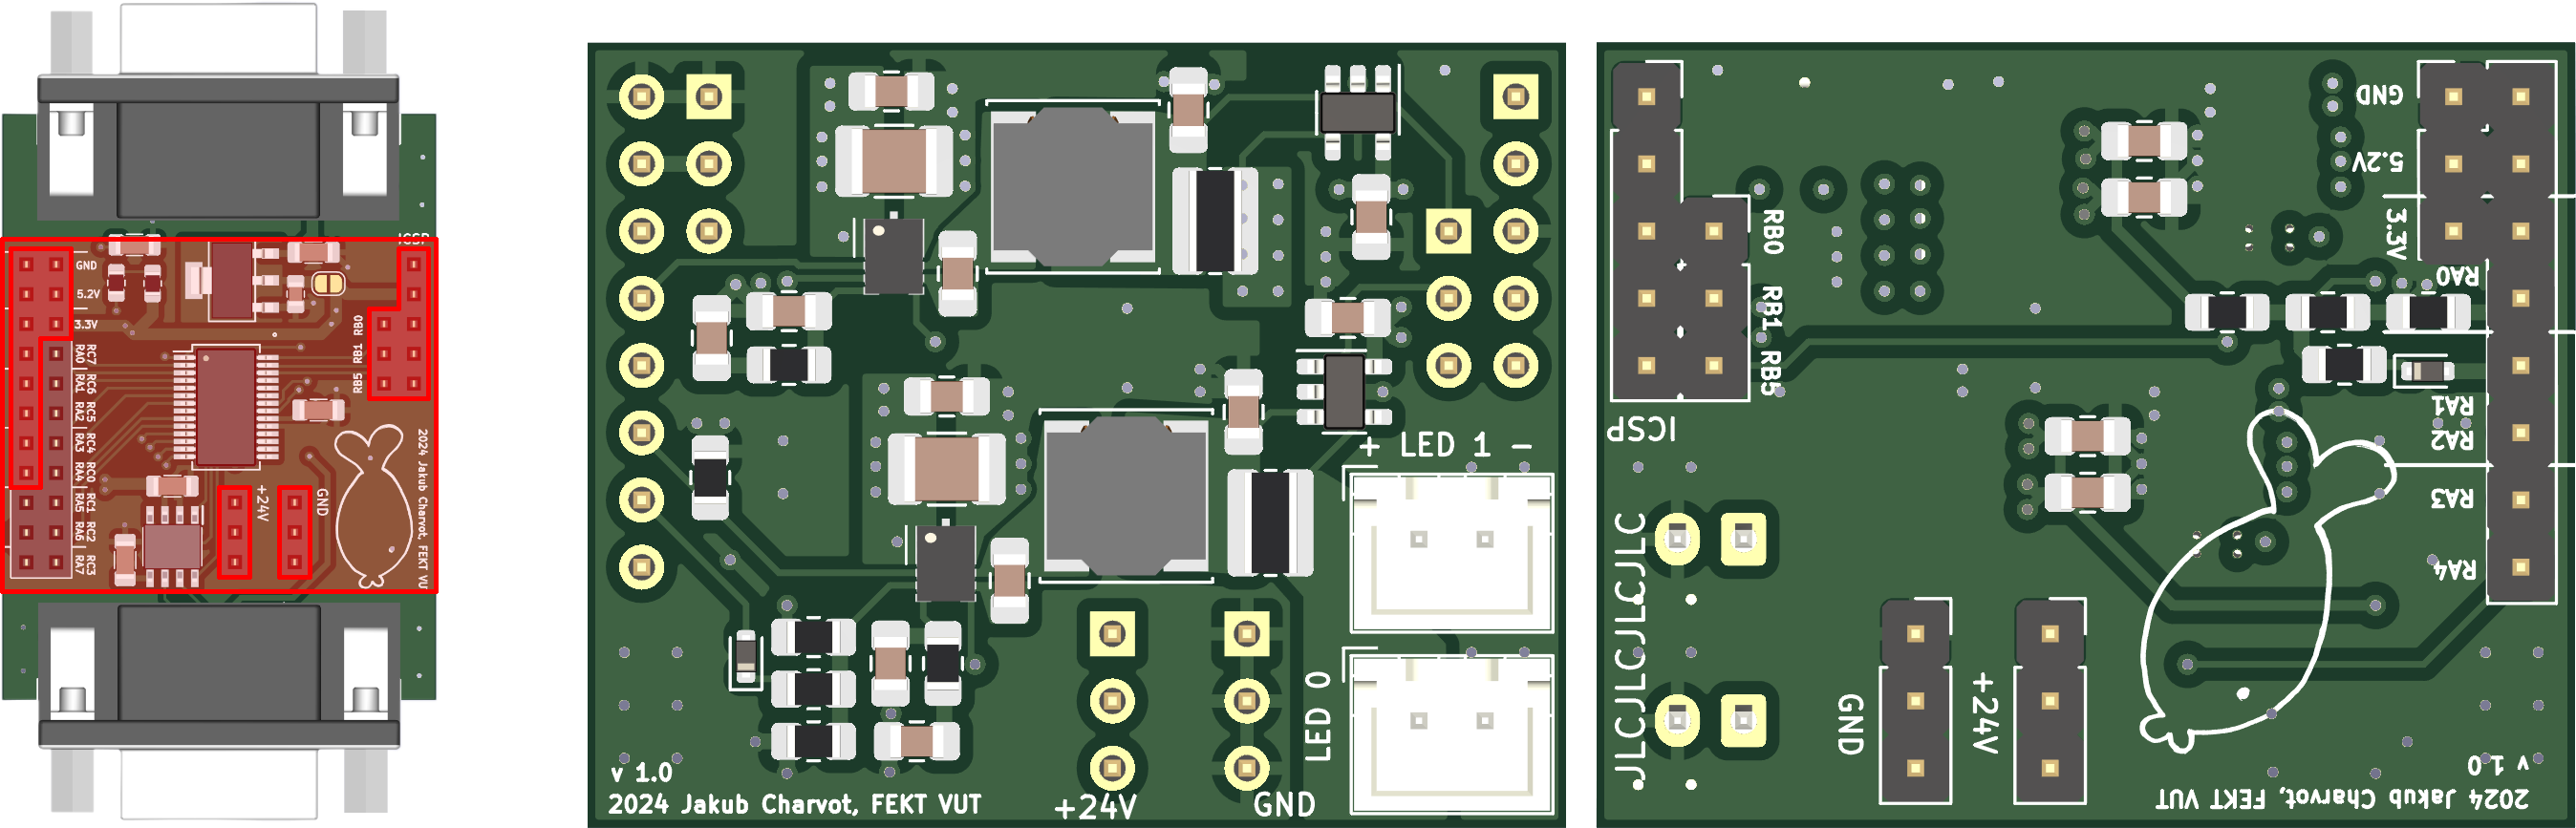
\includegraphics[width=0.8\textwidth]{obrazky/dps/ledboard-combined.png}};
            
            \draw[dashed] (10.1,0.02) -- (12.5,0.02);
            \draw[<->,thick] (12.5,0.02) -- (12.5,3.66);
            \draw[dashed] (12.5,3.66) -- (10.1,3.66);
            \node[anchor=west] at (12.5,1.83)  {\qty{36}{mm}};

            \draw[dashed] (2.75,0.02) -- (2.75,-0.5);
            \draw[<->,thick] (2.75,-0.6) -- (7.3,-0.6);
            \draw[dashed] (7.3,-0.6) -- (7.3,0.02);
            \node[anchor=south] at (5,-0.6)  {\qty{57}{mm}};

            \draw[dashed,thick,color=red] (2.75,0.02) -- (2.05,1.1);
            \draw[dashed,thick,color=red] (2.75,3.66) -- (2.05,2.7);
        \end{tikzpicture}
        \caption{Vizualizace \acs{dps} periferie \acs{led} osvětlení.}
        \label{fig:perif-led-dps}
    \end{figure}

    Za účelem zvětšení plochy pro umístění součástek byly z konektorů obecného modulu vyvedeny pouze některé piny, i přesto bylo nakonec potřeba umístit komponenty také na spodní stranu \acs{dps}. Rozmístění součástek je obdobné pro oba měniče napětí a respektuje doporučení výrobce a tedy i obecná pravidla pro návrh měničů napětí~\cite{Diodes_AP63356Q}. Je kladen důraz na to, aby smyčka ze spínacího uzlu přes výstupní kapacitu a zem zpět do kontroléru byla co nejkratší a vedena za pomoci polygonů. Stejně tak vstupní kapacitor je umístěn přímo vedle vstupních pinů kontroléru.
    